\begin{table}[p]\centering\small\caption{Exact-target certificate economics at the two-second limit.}\label{tab:proof56}
\begin{tabular}{@{}rrrrrrr@{}}\toprule
$k,N$ & Seed & Check seconds & Raw bytes & Gzip bytes & Price bits & Final book \\ \midrule
$8,9$ & 5601 & 0.0096 & 1662 & 512 & 5/5 & 2 \\
$8,9$ & 5602 & 0.0258 & 2275 & 621 & 7/7 & 3 \\
$8,9$ & 5603 & 0.0201 & 2027 & 609 & 16/16 & 2 \\
$24,17$ & 5601 & 0.0539 & 3704 & 709 & 8/7 & 4 \\
$24,17$ & 5602 & 0.0558 & 3743 & 707 & 6/6 & 3 \\
$24,17$ & 5603 & 0.0577 & 3739 & 718 & 8/8 & 3 \\
$96,25$ & 5601 & 0.3770 & 12083 & 1313 & 5/5 & 4 \\
$96,25$ & 5602 & 0.3925 & 12021 & 1284 & 2/1 & 4 \\
$96,25$ & 5603 & 0.3765 & 12190 & 1343 & 7/7 & 4 \\
\bottomrule\end{tabular}
\par\smallskip\begin{minipage}{\textwidth}\footnotesize Both byte counts include the original input model, policy and full proof tree. Gzip uses deterministic zero timestamp; price bits report maxima of absolute numerator and positive denominator over retained leaf prices. Tested-price and distinct-book information is separately available in the mechanical replay.\end{minipage}
\end{table}\clearpage
\begin{figure}[p]\centering
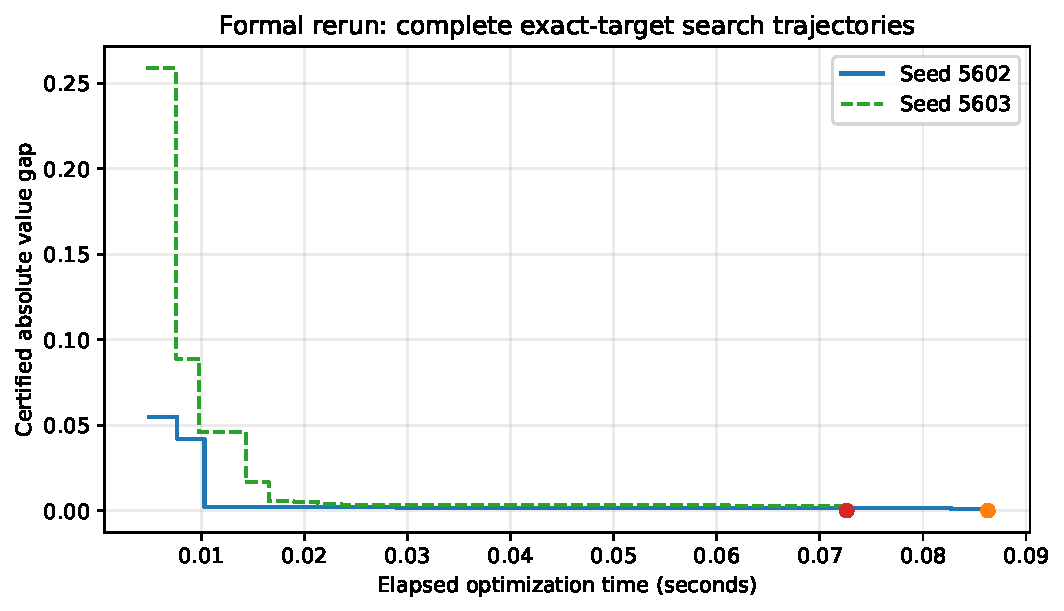
\includegraphics[width=\textwidth]{revisions/or-r58-structural-referee-20260926/generated/exact_trajectories.pdf}
\caption{Complete recorded exact-target price trajectories for the two eight-history instances requiring branching. Every recorded epoch is retained. The final circles denote zero rational width; elapsed times are those of the published two-second-limit runs, not the later mechanical replay.}\label{fig:trajectory56}
\end{figure}\clearpage
